%!TEX TS-program = xelatex
%!TEX encoding = UTF-8 Unicode
%!TEX root = 2023-DP-TTRA.tex
%----------------------------------------------------------------- LANGUAGES ---
\newcommand{\mylanguages}{italian,english} % in reverse order
%---------------------------------------------------------- TITLE & SUBTITLE ---
\newcommand{\mytitle}{Tecniche di Ripresa e Registrazione Audio}
\newcommand{\mysubtitle}{Pratiche sperimentali di registrazione dell'organo a canne, \\ differenti approcci di ripresa del suono}
%----------------------------------------------------------------- AUTHOR(s) ---
\newcommand{\authorone}{Doralma A. Palestra}
\newcommand{\institutione}{Conservatorio N. Piccinni di Bari}
\newcommand{\emailone}{doralma.palestra@gmail.com}
%-------------------------------------------------------------------------------


%-------------------------------------------------------------- STYLE GS2020 ---
%!TEX TS-program = xelatex
%!TEX encoding = UTF-8 Unicode
%!TEX root = 2022-GS-ARTICLE.tex
%-------------------------------- PACKAGES AND OTHER DOCUMENT CONFIGURATIONS ---
\documentclass[
	a4paper,
	twocolumn,
	twoside,
	%openright
]{article}
\usepackage[
	top=20mm,
	bottom=25mm,
	textwidth=17.2cm,
	columnsep=0.8cm,
	bindingoffset=1cm,
	%showframe
]{geometry}
\usepackage[T1]{fontenc}
\usepackage[\mylanguages]{babel}
\usepackage{csquotes}
%\usepackage{parskip}
\usepackage[style=authoryear-ibid,backend=biber]{biblatex}
\bibliography{includes/bibliography.bib}
\usepackage{dblfloatfix}
\usepackage{subfigure}
\usepackage[subfigure]{tocloft}
\advance\cftsecnumwidth 0.5em\relax
\advance\cftsubsecindent 0.5em\relax
\advance\cftsubsecnumwidth 0.5em\relax
\usepackage{graphicx}
\usepackage{wrapfig}
% \usepackage{epstopdf}
% \epstopdfsetup{update}
\usepackage[usenames]{color}
\usepackage{xcolor}
\usepackage{tikz}
\usetikzlibrary{shapes,
                through,
								calc,
								intersections,
								backgrounds,
                positioning}
\usepackage{tkz-euclide}
\usepackage{amssymb}
\usepackage[
  colorlinks=true,
  linkcolor=black,
	anchorcolor=black,
	citecolor=black,
	filecolor=black,
	menucolor=black,
	runcolor=black,
	urlcolor=black
	]{hyperref}
\usepackage{Alegreya}
\linespread{1.05}
\usepackage{
	fontspec,
	xltxtra,
	xunicode
	}
\usepackage{
	xfrac,
	unicode-math
	}

\defaultfontfeatures{Mapping=tex-text}
\setmonofont[
	Scale=MatchLowercase
	]{Andale Mono}
\setmathfont[
	Scale=MatchLowercase,
	Scale=1
	]{Libertinus Math}

\usepackage{microtype}

\usepackage[
	hang,
	small,
	labelfont=bf,
	up,
	textfont=it,
	up
	]{caption}
\usepackage{paralist} % For compact item lists
\usepackage{etoolbox} % Some tools: used for quote environment
\AtBeginEnvironment{quote}{\small}
\usepackage{titling} % Customizing the title section
\usepackage{booktabs} % Horizontal rules in tables
\usepackage{enumitem} % Customized lists
\setlist[itemize]{noitemsep} % Make itemize lists more compact
\usepackage{abstract} % Allows abstract customization
\renewcommand{\abstractnamefont}{\normalfont\bfseries} % Set the "Abstract" text to bold
\renewcommand{\abstracttextfont}{\normalfont\small\itshape} % Set the abstract itself to small italic text
\usepackage{titlesec} % Allows customization of titles
\renewcommand\thesection{\Roman{section}} % Roman numerals for the sections
\renewcommand\thesubsection{\Roman{subsection}} % roman numerals for subsections
\titleformat{\section}[block]{\Large}{\thesection.}{1em}{} % Change the look of the section titles
\titleformat{\subsection}[block]{\large}{\thesubsection.}{1em}{} % Change the look of the section titles
%------------------------------------------------------------- TITLE SECTION ---
\setlength{\droptitle}{-4\baselineskip} % Move the title up
\pretitle{\begin{center}\huge\bfseries} % Article title formatting
\posttitle{\end{center}} % Article title closing formatting
\title{\mytitle \\[0.1cm] \large{\emph{\mysubtitle}}} % Article title
\author{%
\textsc{\authorone}\\%
\normalsize \institutione \\ %
\normalsize \emailone %
% activate
% \and % duplicate these 4 lines if more
% \textsc{\authortwo} \\%
% \normalsize \institutiontwo \\ %
% \normalsize \emailtwo %
}
\date{} % Leave empty to omit a date

\usepackage{fancyhdr} % Headers and footers
\pagestyle{fancy} % All pages have headers and footers
\fancyhead{} % Blank out the default header
\fancyfoot{} % Blank out the default footer
\fancyhead[C]{\small Wikipedia • General Relativity} % Custom header text
\fancyfoot[RO]{\small \today~ • w: \input{includes/words.txt} • c: \input{includes/char.txt} • p:~\thepage} % Custom footer text
\fancyfoot[LE]{\small p:~\thepage~ • c: \input{includes/char.txt} • w: \input{includes/words.txt} • \today} % Custom footer text

%-------------------------------------------------------------------------------
%-------------------------------------------------------------------------------
%	LISTINGS
%-------------------------------------------------------------------------------
%-------------------------------------------------------------------------------
\usepackage{listings}
% lstlistings setup
\definecolor{gsbg}{rgb}{0.98,0.98,0.98}

\lstset{%
  aboveskip=10pt,
	belowskip=5pt,
  language=C++,
  numbers=none,%left,%none,
  tabsize=4,
  %frame=single,
  breaklines=true,
  numberstyle=\tiny\ttfamily,
  backgroundcolor=\color{gsbg},
  basicstyle=\footnotesize\ttfamily,
  %commentstyle=\slshape\color{mylstcmt}, %\itshape,
  %frameround=tttt,
  columns=flexible, %fixed,
  showstringspaces=false,
  emptylines=2,
  inputencoding=utf8,
  extendedchars=true,
  literate=	{á}{{\'a}}1
			{à}{{\`a}}1
			{ä}{{\"a}}1
			{â}{{\^a}}1
			{é}{{\'e}}1
			{è}{{\`e}}1
			{ë}{{\"e}}1
			{ê}{{\^e}}1
			{ï}{{\"i}}1
			{î}{{\^i}}1
			{ö}{{\"o}}1
			{ô}{{\^o}}1
			{è}{{\`e}}1
			{ù}{{\`u}}1
			{û}{{\^u}}1
			{ç}{{\c{c}}}1
			{Ç}{{\c{C}}}1,
  emph={component, declare, environment, import, library, process},
  emph={[2]ffunction, fconstant, fvariable},
  emph={[3]button, checkbox, vslider, hslider, nentry, vgroup, hgroup, tgroup, vbargraph, hbargraph, attach},
  %emphstyle=\color{yotxt}, %\underline, %\bfseries,
  %morecomment=[s][\color{mylstdoc}]{<mdoc>}{</mdoc>},
  rulecolor=\color{black}
}

\usepackage[framemethod=tikz]{mdframed} % Allows defining custom boxed/framed environments

%-------------------------------------------------------------------------------
%--------------------------------------------------- INFORMATION ENVIRONMENT ---
%-------------------------------------------------------------------------------

% Usage:
% \begin{info}[optional title, defaults to "Info:"]
% 	contents
% 	\end{info}

\mdfdefinestyle{info}{%
	topline=false, bottomline=false,
	leftline=false, rightline=false,
	nobreak,
	singleextra={%
		\fill[black](P-|O)circle[radius=0.4em];
		\node at(P-|O){\color{white}\scriptsize\bf i};
		\draw[very thick](P-|O)++(0,-0.8em)--(O);%--(O-|P);
	}
}

% Define a custom environment for information
\newenvironment{info}[1][Info:]{ % Set the default title to "Info:"
	\medskip
	\begin{mdframed}[style=info]
		\footnotesize\noindent{\textbf{#1}}
}{
	\end{mdframed}
}

%-------------------------------------------------------------------------------
%----------------------------------------------------- BIOGRAFIA ENVIRONMENT ---
%-------------------------------------------------------------------------------

% Usage:
% \begin{bio}[optional title, defaults to "Info:"]
% 	contents
% 	\end{bio}

\mdfdefinestyle{bio}{%
	topline=false, bottomline=false,
	leftline=false, rightline=false,
	nobreak,
	singleextra={%
		\fill[black](P-|O)circle[radius=0.4em];
		\node at(P-|O){\color{white}\scriptsize\bf b};
		\draw[very thick](P-|O)++(0,-0.8em)--(O);%--(O-|P);
	}
}

% Define a custom environment for information
\newenvironment{bio}[1][Biografia:]{ % Set the default title to "Info:"
	\medskip
	\begin{mdframed}[style=bio]
		\noindent{\textbf{#1}}
}{
	\end{mdframed}
}

%-------------------------------------------------------------------------------
%------------------------------------------------------- WARNING ENVIRONMENT ---
%-------------------------------------------------------------------------------

% Usage:
% \begin{warn}[optional title, defaults to "Warning:"]
%	Contents
% \end{warn}

\mdfdefinestyle{warning}{
	topline=false, bottomline=false,
	leftline=false, rightline=false,
	nobreak,
	singleextra={%
		\draw(P-|O)++(-0.5em,0)node(tmp1){};
		\draw(P-|O)++(0.5em,0)node(tmp2){};
		\fill[black,rotate around={45:(P-|O)}](tmp1)rectangle(tmp2);
		\node at(P-|O){\color{white}\scriptsize\bf !};
		\draw[very thick](P-|O)++(0,-1em)--(O);%--(O-|P);
	}
}

% Define a custom environment for warning text
\newenvironment{warn}[1][Warning:]{ % Set the default warning to "Warning:"
	\medskip
	\begin{mdframed}[style=warning]
		\noindent{\textbf{#1}}
}{
	\end{mdframed}
}

%-------------------------------------------------------------------- ABSTRACT -
\renewcommand{\maketitlehookd}{%
\begin{abstract}
\noindent\input{includes/abstract.txt}
\end{abstract}
}

%------------------------------------------------------------ BEGIN DOCUMENT ---
\begin{document}
\maketitle TECNICHE DI REGISTRAZIONE
\thispagestyle{empty}
%-------------------------------------------------------------------- ABSTRACT -
% The abstract is an external txt file inside the includes folder
%-------------------------------------------------------------------------------
\section*{Per una ripresa dell'organo a canne}
dotato della sua complessità timbrica e spaziale, 
gli approcci possono essere molteplici e differenziati.
Da una rappresentazione stereofonica che si àncora ad un punto di 
vista ideale a livello di palco, fino ad una ripresa spaziata con tecnica 
ambisonica.

\section*{Spazio sonoro}
Il dato spaziale è fondamentale nell'esperienza d'ascolto. La complessità
 timbrica propria dell'organo necessita di uno spazio sonoro adeguato. 
 Riguardo l'incisione dei suoni su supporto, la molteplicità delle 
 interpretazioni possibili ha restituito differenti approcci, i quali 
 rappresentano il suono in modi differenti tramite diverse configurazioni
  spaziali dei set microfonici.   %-------------------------------------------------------------------------------
\subsection*{Immagini sonore}
Le differenti configurazioni assunte durante la registrazione restituiscono 
dati sonori influenzati dal parametro spazio.
La distanza dei microfoni dalla fonte sonora, determina un filtraggio dello 
spettro sonoro, includendo elementi spaziali quali onde riflesse e coda 
riverberante propria del luogo.
La registrazione presa in esame riguarda l'organo a canne dell'Auditorium 
del Conservatorio N. Piccinni di Bari.

\begin{warn}[Differenti approcci: spazio e timbro]
La scelta dei microfoni,- conoscendo le corrispondenti figure polari,- e del 
loro posizionamento nello spazio, -distanza dalla sorgente, spazialità interna 
al set microfonico, - costituiscono una scelta di rappresentazione del suono.
Ogni configurazione restituisce uno o più punti dello spazio, e dunque una 
specifica condizione d'ascolto.

\end{warn}


Per la ripresa audio sono stati creati tre set microfonici, con intenti e 
possibilità di resa sonora specifiche. %-------------------------------------------------------------------------------

\subsubsection*{Set Microfonici}
La prima configurazione rappresenta un'immagine stereofonica che 
rimarca la linea di palco, attraverso l'utilizzo di quattro canali:
una coppia spaziata AB (chnls 3, 4) di microfoni ominidrezionali 
(OM1- casa Line Audio), un setup ORTF, naturalmente costituito da 
microfoni cardioidi (casa Schoeps).
Il secondo setup di microfoni restituisce un'immagine ambisonica, prodotta 
da quattro Omnidirezionali (OM1) disposti sulle facce di un tetraedro.
La terza configurazione rappresenta un setup simile nella disposizione 
delle capsule microfoniche, con una ripresa effettuata mediante sistema 
SoundField, costituito invece da quattro sub-cardioidi.

Le configurazioni microfoniche qui esposte sono state disposte ad una 
distanza: adeguata alla timbrica dell'organo, coerente all'acustica e alle 
risonanze della sala, ottimizzata rispetto al tipo di microfoni e di setup 
predisposto.

\begin{figure}[b]
\begin{center}
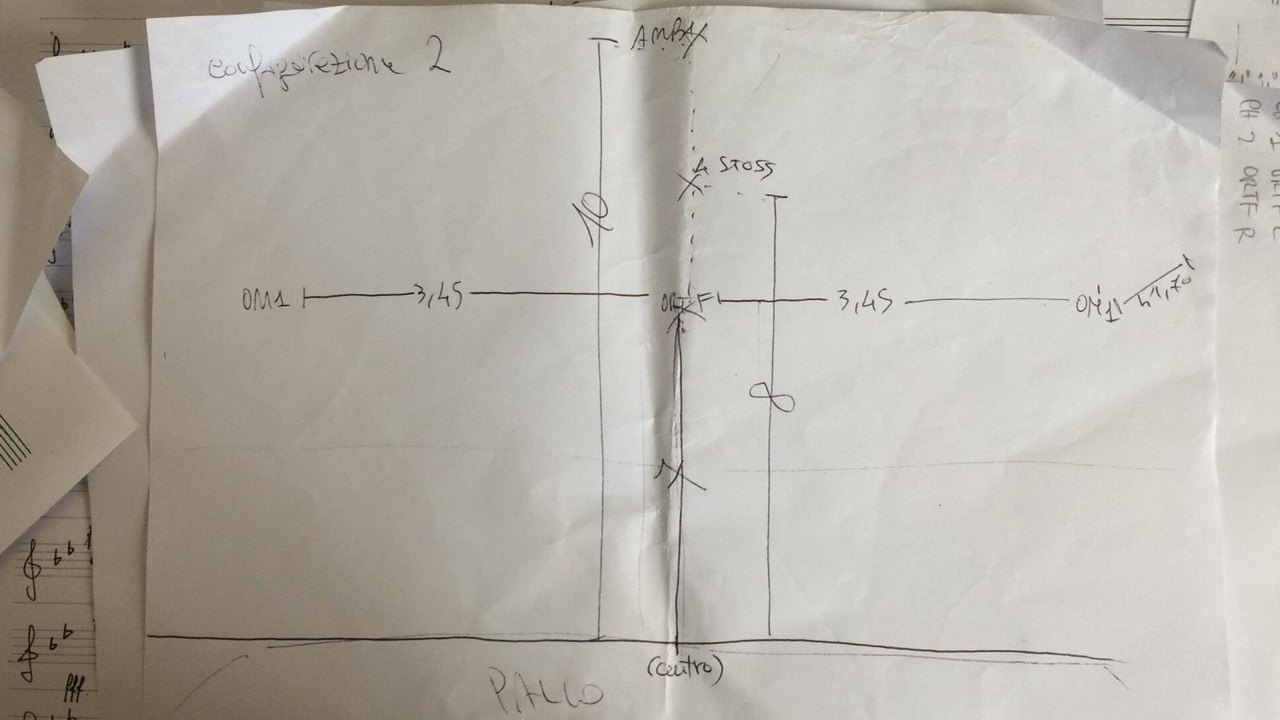
\includegraphics[width=.47\textwidth]{img/img0.jpeg}
\caption{\textbf{}. 
\label{gr01}
\end{center}
\end{figure}



\section*{Strumenti di ascolto spaziale}
L'esperienza sonora si lega per sua natura allo spazio in cui si diffondono 
gli eventi. Disporre di molteplici registrazioni, effettuate a diverse distanze
dalla fonte sonora, consente di effettuare operazioni 'impossibili', per poter 
studiare i risultati sonori e compararli.

\subsubsection*{MidSide per il Frontepalco}
Per la rappresentazione 'frontale', si sceglie un trattamento dell'immagine 
stereo tramite il metodo MS (MidSide), in cui i canali Left e Right vengono 
posti in relazione a creare un'immagine che non presenta problemi di fase,
e che mette in relazione il suon diretto (Mid) con il suono ambientale (Side).
E' possibile applicare questa configurazione alla coppia spaziata AB e al setup 
ORTF, tramite vst progettato in Faust.


\begin{lstlisting}
mspan(x,p,rad) = m,s
with{
  m = (p*x)+((1-p)*(x*cos(rad)));
  s = x*(sin(-rad));
};
\end{lstlisting}

\begin{figure}[b]
\begin{center}
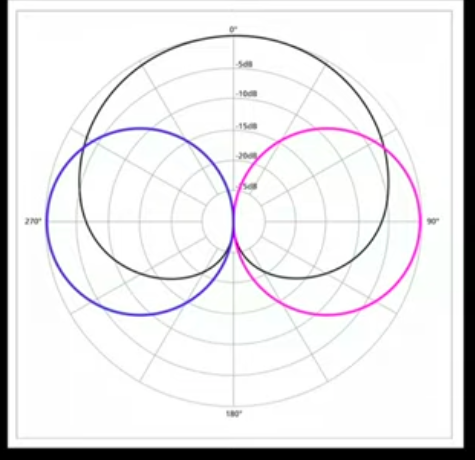
\includegraphics[width=.47\textwidth]{img/img7.png}
\caption{\textbf{}. 
\label{gr01}
\end{center}
\end{figure}


Questa prima configurazione, seppure descritta come frontale, 
riporta all'interno del segnale la componente spaziale, fondamentale per la 
rappresentazione dell'organo a canne.


\subsubsection*{Immagine stereo sferica}

Le due restanti configurazioni impiegano microfoni disposti sulle facce di un 
tetraedro, per restiruire un'immagine stereo tridimensionale.
Secondo questa logica, un gradiente di pressione omnidirezionale W agisce 
sulle coordinate forntali dell'asse X, su quelle coordinate verticali sull'asse Z 
e sulle coordinate orizzontali che corrono sull'asse Y.

\begin{figure}[b]
\begin{center}
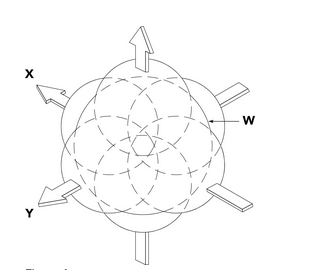
\includegraphics[width=.47\textwidth]{img/img10.png}
\caption{\textbf{}. 
\label{gr01}
\end{center}
\end{figure}

I dati che corrispondo al segnale ambisonico,- forniti dalla prima configurazione 
attraverso un dispositivo soundfield (4 subcardioidi, che generano 3 figure a 8), 
o da un terzo dispositivo tetraedrico dotato di quattro omindirezionali, - sono 
distinti quali A-format.

I quattro segnali ripresi dai microfoni in A-format (ambiosonico del secondo ordine), 
sono da decodificare in B format (ambiosonico del terzo ordine), in cui i segnali 
saranno combinati a formare una figura omnidirezionale e tre figure a 8.
Tale decodifica consente di assegnare figure polari e combinarle successivamente 
in numero e combinazioni differenti, anche dopo la registrazione, tramite dsp. 
E' possibile, ad esempio, generare da quattro segnali otto canali.
In questo modo, il microfono soundfiled, o il dispositivo tetraedrico non rappresenta
solo una di coppie coincidenti ravvicinate, che creano 3 figure a 8, con gradiente
di pressione sferico, ma costituiscono la base di un lavoro creativo e sperimentale
molto più vasto.

\begin{figure}[b]
\begin{center}
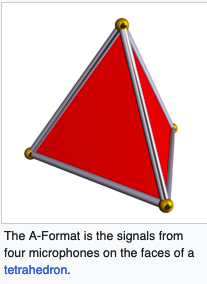
\includegraphics[width=.47\textwidth]{img/img9.png}
\caption{\textbf{}. 
\label{gr01}
\end{center}
\end{figure}


\begin{lstlisting}
atobformat(x,y,z,w) = X,Y,Z,W
with{
  X = 0.5((LF–LB) + (RF–RB));
 Y = 0.5((LF–RB) – (RF–LB);
  Z = 0.5((LF–LB) + (RB–RF));
   W = 0.5(LF+LB+RF+RB);
};
\end{lstlisting}

In conclusione, la ripresa soundfield può essere considerata come una 
naturale estensione della logica Mid-Side, dove i segnali che viaggiano 
su differenti canali vengono posti in relazione e manipolati per gestire 
l'immagine stereo.

Il MidSide consente di allargare o stringere l'immagine stereo, focalizzando
il missaggio dei segnali sulla sorgente, o viceversa sullo spazio risonante.
Il setup Ambisonico consente di manipolare il punto di ascolto nello spazio, 
gestendo la compjnente delle coordinate dello spazio tridimensionale.


      
 \subsection*{Muovere le distanze}
 Uno strumento utile per comprendere l'approccio ad un ascolto delle 
 caratteristiche risonanti de luoghi, e in conseguenza al filtraggio che 
 lo spazio stesso effettua sul timbro, è l'osservazione e l'ascolto,
 dei differetni risultati sonori rappresentati dalle differenti configurazioni.
 
 E' possibile parlare anche di ambiente ambisonico ibrido, quando si impiega
 per la ripresa un ORTF accanto al SoundField.
 
 La possibilità di ravvicinare la fonte sonora, includere la componente spaziale
 più o meno rispetto al segnale ripreso in fase di registrazione, sono operazioni
 che derivano dalla logica del MidSide e della gestione dell'immagine stereo,
tramite signal processing, ad oggi digitale.

Poter modificare il punto di ascolto, gestire le risonanze, dedicando ad ogni
componente un canale adeguato, permette di restituire un suono che sia il 
risultato delle scelte consapevoli, e dunque artistiche, di chi conduce la registrazione.

La possibilità do avvalersi di una ripresa tridimensionale amplifica l'area di azione
dell'autore della ripresa microfonica. 



 
\section*{Conclusioni}
  In definitiva, la ripresa di un segnale audio, richiede abilità tecniche che non restano 
  tuttavia mero tecnicismo, ma riflettono una scelta artistica guidata dalla precisa 
  interpretazione del suono e della perfomance in registrazione.
  
  Le tecniche di ripresa e registrazione, sono il passo precedente al trattamento del 
  segnale audio, ma ancora entro il processo creativo di rappresentazione del suono.
  
  Se la musica è linguaggio delle emozioni, la restituzione su supporto degli eventi
  sonori si fa interprete di quel linguaggio che, a seconda del pensiero che lo supporta, 
 assume un vocabolario, una punteggiatura e un'intenzione specifica e inscindibile dal 
 risultato finale, che sarà quello che segnerà il significato ultimo del discorso, quello che 
 arriverà a scandire il tempo del fruitore.
\vfill\null



\newpage % USE NEWPAGE TO FORCE COLUMNN INTERRUPTION
%-------------------------------------------------------------------------------
%-------------------------------------------------------------------------------


\begin{quote}
La musica non e` solo composizione. \\
Non è artigianato, non è un mestiere. \\
La musica è pensiero. \cite{nono85}
\end{quote}




%\begin{figure}[t]
%\centering
%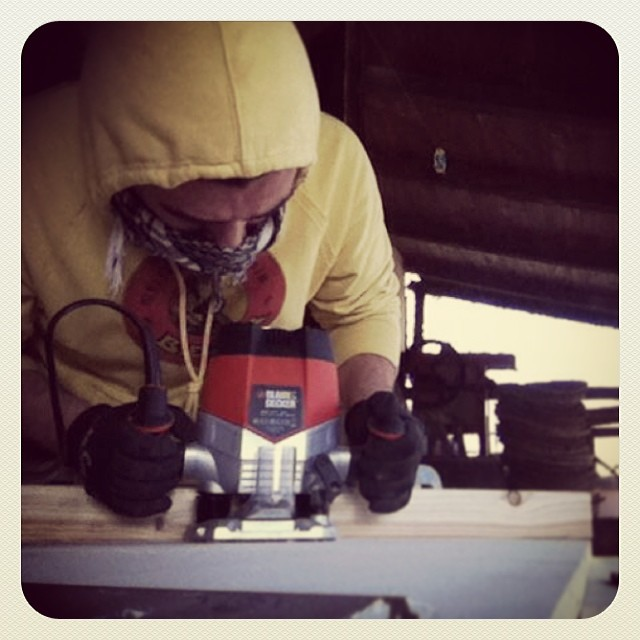
\includegraphics[width=.47\textwidth]{img/image2.jpg}
%\caption{Mic Mapping}
%\label{gs}
%\end{figure}

%\begin{equation}
%m(x,p,\theta) = (p*x) + ((1-p)*(x\cos\theta)
%\label{eq:mid}
%\end{equation}
%
%Some predictions of general relativity differ significantly from those of
%classical physics, especially concerning the passage of time, the geometry of
%space, the motion of bodies in free fall, and the propagation of light.

%--------------------------------------------
%----------------larghezza massima del codice
%\begin{lstlisting}
%mspan(x,p,rad) = m,s
%with{
%  m = (p*x)+((1-p)*(x*cos(rad)));
%  s = x*(sin(-rad));
%};
%\end{lstlisting}
%
%Examples of such differences include gravitational time dilation, gravitational
%lensing, the gravitational redshift of light, and the gravitational time delay.
%The predictions of general relativity in relation to classical physics have been
%confirmed in all observations and experiments to date.

\vfill\null

\raggedright
\bibliographystyle{unsrt}
\printbibliography


\end{document}

%%%%%%%%%%%%%%%%%%%%%%%%%%%%%%%%%%%%%%%%%%%%%%%%%%%%%%%%%%%%%%%%%%%%%%%%%%%%%%%%
% 2020 GIUSEPPE SILVI ARTICLE TEMPLATE BASED ON
%%%%%%%%%%%%%%%%%%%%%%%%%%%%%%%%%%%%%%%%%%%%%%%%%%%%%%%%%%%%%%%%%%%%%%%%%%%%%%%%
% Journal Article
% LaTeX Template
% Version 1.4 (15/5/16)
% This template has been downloaded from:
% http://www.LaTeXTemplates.com
% Original author:
% Frits Wenneker (http://www.howtotex.com) with extensive modifications by
% Vel (vel@LaTeXTemplates.com)
% License:
% CC BY-NC-SA 3.0 (http://creativecommons.org/licenses/by-nc-sa/3.0/)
%%%%%%%%%%%%%%%%%%%%%%%%%%%%%%%%%%%%%%%%%%%%%%%%%%%%%%%%%%%%%%%%%%%%%%%%%%%%%%%%
